% \renewcommand{\ldate}{2016-01-}
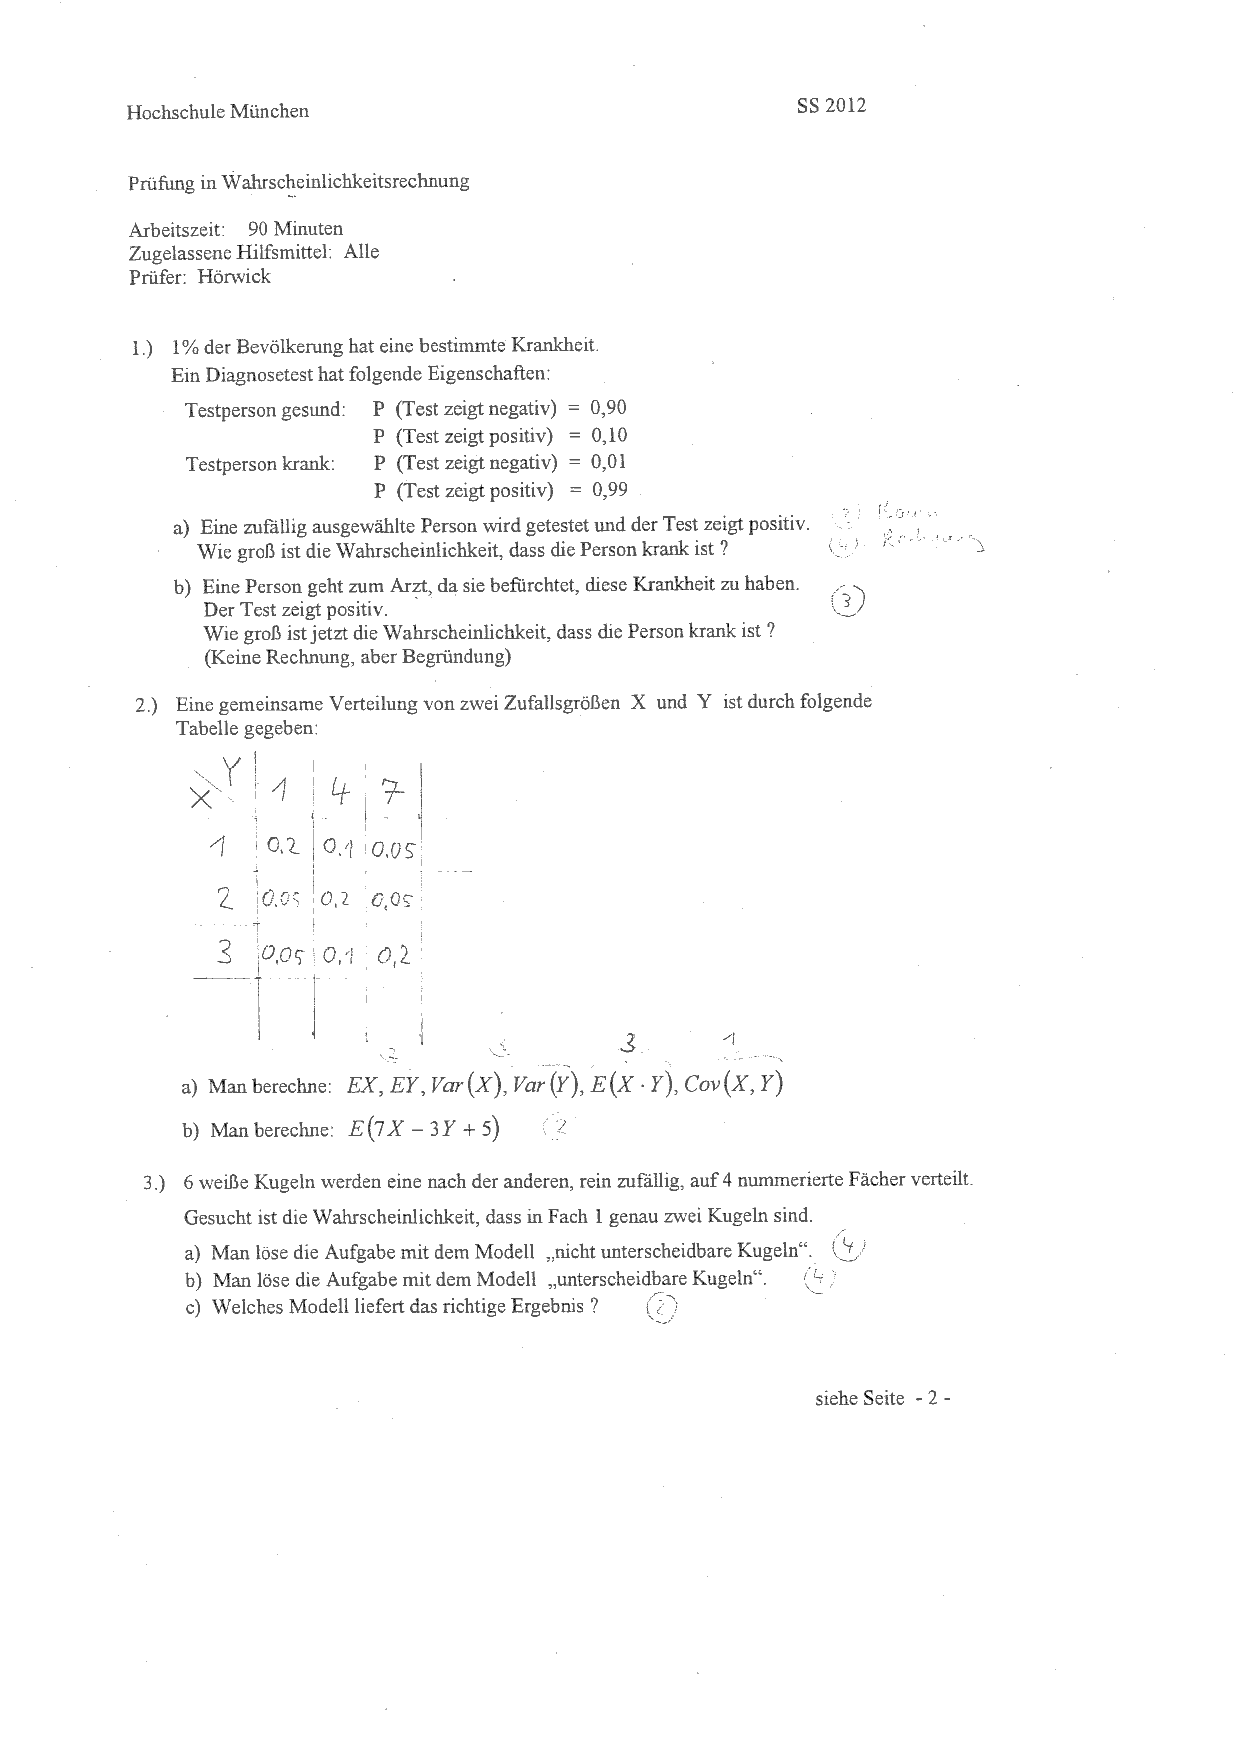
\includepdf[pages=-]{pruefungsangabe_wahrStat_ss2012}

\section{Lösung für die Prüfung SS 2012}

\subsection{zu 1)}
%1 \includegraphicsdeluxe{baumZuSs20121.jpg}{Wahrscheinlichkeitsbaum}{Wahrscheinlichkeitsbaum}{fig:baumZuSs20121}

\subsubsection{zu 1a)}
A: Person krank\\
B: Test zeigt positiv
$P(A|B) = \frac{P\cap B}{P(B)} = \frac{0.01\cdot 0.99}{0.01\cdot 0.99 + 0.99\cdot 0.10} = 0.09$

\subsubsection{zu 1b)}
Jetzt ist die apriori Wahrscheinlichkeit, dass er krank ist, höher (vielleicht 0.1 statt 0.01). Damit ist die aposteriori Wahrscheinlichkeit, dass er krank ist, auch höher (vielleicht 0.5). 

\subsection{zu 2a)}